\chapter{Extremos relativos}
\section{Extremos relativos}

\begin{defi}
Sea $U\subset\R^n$ abierto, sea $\function{f}{U}{\R}$ y sea $a\in U$, diremos que $a$ es:
\begin{itemize}
\item Punto máximo relativo de $f$ si $\exists r>0\talque f(x)\leq f(a)\ \forall x\in B(a,r)$.
\item Punto mínimo relativo de $f$ si $\exists r>0\talque f(x)\geq f(a)\ \forall x\in B(a,r)$.
\item Punto de extremo relativo de $f$ si es un punto máximo o mínimo relativo.
\end{itemize}
\end{defi}

\begin{proposicion} Sea $U\subset\R^n$ abierto, sea $\function{f}{U}{\R}$ y sea $a\in U$. Si $f$ tiene un extremo relativo en $a$, y $f$ es diferenciable en $a$, entonces $df(a)=0$ (ó equiv. $\gradiente f(a)=\overline{0}$).
\begin{proof}\ \\
Por hipótesis $\exists r>0\talque f(a)$ es máx. o mín. de $f$ en $B(a,r)$. Fijado un $i\in\{1,2,...,n\}$, la función $\varphi(t)=f(a+te_i)$ tiene máx. o mín. relativo en $t=0$. Sea $\Phi(t)=a+te_i\talque \varphi=f\circ\Phi$. Por la \textit{regala de la cadena} $\varphi$ es diferenciale en $t=0$ y por el \textit{teorema del extremo interior} tenemos que $\varphi'(0)=0$, luego $0=\varphi'(0)=\dotproduct{\gradiente f(\Phi(0))}{\Phi'(0)}=\dotproduct{\gradiente f(a)}{e_i}=\\
=D_if(a)$. Luego $D_i f(a)=0\ \forall i\in\{1,2,...,n\}\implies \gradiente f(a) = 0$ y por ser $f$ diferenciable en $a$, $D_uf(a)=0\ \forall u\in\R^n$ con $\norm{u}=1$.
\end{proof}
\end{proposicion}

\begin{defi} Sea $U\subset\R^n$ abierto y sea $\function{f}{U}{\R}$. Diremos que $a\in U$ es punto crítico de $f$ si $df(a)=0$ (ó equiv. $\gradiente f(a)=\overline{0}$).
\end{defi}

\begin{observacion} $a$ punto crítico de $f\nimplies a$ punto de extremo relativo de $f$.
\begin{ejem} $0$ en $f(x)=x^3$ es punto crítico pero no relativo.\end{ejem} 
\end{observacion}

\begin{nota} Sea $\function{f}{U\subset\R^n}{\R}$, si $n\geq 2$, a los puntos críticos que no son puntos relativos los denominamos puntos de silla.\\\end{nota}
\begin{figura}\ \\
	\begin{center}
	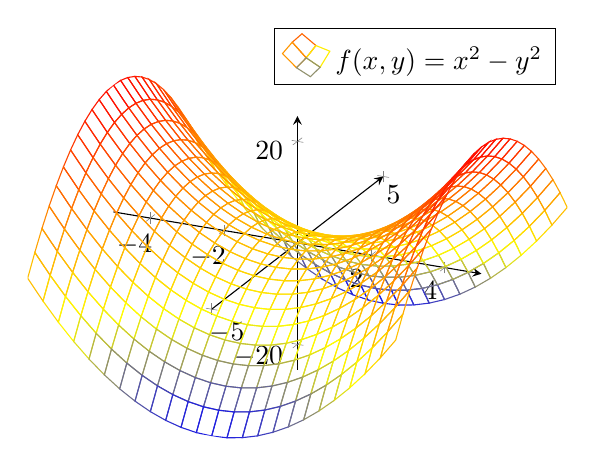
\begin{tikzpicture}
	\begin{axis} [axis lines=middle]
	\addplot3[mesh,colormap/hot, domain=-5:5]{x^2-y^2};\addlegendentry{$f(x,y)=x^2-y^2$}
	%\addplot3 ({0},{0},{0}); \addlegendentry{$(0,0,0)$}
	\end{axis}
	\end{tikzpicture}
	\end{center}
	Punto de silla en $f(0,0)=0$.
\end{figura}

\begin{proposicion} Una aplicación del \textit{teorema de Taylor} es que nos aporta información sobre cuando un punto crítico es punto de extremo relativo.\\
Sea $U\subset\R^n$ abierto, sea $\function{f}{U}{\R}$, con $f\in C^2(U)$ y sea $a\in U$. Si $a$ es punto crítico de $f$ ($df(a)=0$), tenemos (si $B(a,r)\subset U$) que $\forall x\in B(a,r)\ \exists c_x\in[a,x]\talque f(x)=\\
=\underset{P_{1,a}(x-a)}{\underbrace{f(a)+df(a)(x-a)}}+\underset{R_{1,a}(x-a)}{\underbrace{\dfrac{1}{2!}\left(\stackbin[i,j=1]{n}\sum(x_i-a_i)(x_j-a_j)D_{ij}f(c_x)\right)}}\overset{df(a)=0}=\\
=f(a)+\dfrac{1}{2!}\left(\stackbin[i,j=1]{n}\sum(x_i-a_i)(x_j-a_j)D_{ij}f(c_x)\right)\implies\\
\implies f(x)-f(a)=\dfrac{1}{2!}\left(\stackbin[i,j=1]{n}\sum(x_i-a_i)(x_j-a_j)D_{ij}f(c_x)\right)$.\\
Si $a$ es punto de máximo relativo de $f$, entonces $\exists\delta>0\ (\delta\leq r)\talque f(x)-f(a)\leq 0\\
\forall x\in B(a,\delta)$. Y por tanto, $\stackbin[i,j=1]{n}\sum (x_i-a_i)(x_j-a_j)D_{ij}f(c_x)\leq 0\ \forall x\in B(a,\delta)$. Y así, como $D_{ij}f$ e continua en $a$ tenemos que $\stackbin[i,j=1]{n}\sum (x_i-a_i)(x_j-a_j)D_{ij}f(a)\leq 0$ puesto que $c_x\overset{x\to a}\longrightarrow a$. Tenemos ahora:\\
$\stackbin[i,j=1]{n}\sum h_ih_jD_{ij}f(a)\leq 0$ con $\norm{h}<\delta$. Y de aquí deducimos que $\stackbin[i,j=1]{n}\sum (th_i)(th_j)D_{ij}f(a)=\\
=t^2\left(\stackbin[i,j=1]{n}\sum h_ih_jD_{ij}f(a)\right)\leq 0\ \forall t\in\R\implies\stackbin[i,j=1]{n}\sum h_ih_jD_{ij}f(a)\leq 0\ \forall h\in\R^n$.
\end{proposicion}

\begin{defi} La matriz $\begin{pmatrix}
	D_{11}f(a) & D_{21}f(a) & \ldots & D_{n1}f(a)\\ D_{12}f(a)& \ddots & &\vdots\\ \vdots & & \ddots & \vdots\\ D_{1n}f(a)& \ldots & \ldots & D_{nn}f(a)\end{pmatrix}$ es la matriz de derivadas parciales segundas de $f$ en $a$. La denominamos matriz \textit{Hessiana} de $f$ en $a$ y la denotamos por $H_f(a)=(D_{ij}f(a))^n_{i,j=1}$.
\end{defi}

\begin{observacion}\ \\
$\stackbin[i,j=1]{n}\sum h_ih_jD_{ij}f(a)=\begin{pmatrix} h_1 & h_2 &\ldots & h_n\end{pmatrix}
\begin{pmatrix}	D_{11}f(a) & D_{21}f(a) & \ldots & D_{n1}f(a)\\ D_{12}f(a)& \ddots & &\vdots\\ \vdots & & \ddots & \vdots\\ D_{1n}f(a)& \ldots & \ldots & D_{nn}f(a)\end{pmatrix}
\begin{pmatrix} h_1 \\ h_2 \\ \vdots \\ h_n\end{pmatrix}$
\end{observacion}

\begin{nota} Antes de continuar conviene leer el Apéndice \textsc{B. Repaso de formas cuadráticas}.\end{nota}

\begin{proposicion} Sea $U\subset\R^n$ abierto, sea $\function{f}{U}{\R}$, $f\in C^2(U)$ y sea $a\in U$ punto crítico de $f$. Entonces:
\begin{enumerate}[1)]
\item $a$ es punto de máximo relativo$\implies Q_{H_f(a)}$ es semidefinida negativa.
\item $a$ es punto de mínimo relativo$\implies Q_{H_f(a)}$ es semidefinida positiva.
\item $Q_{H_f(a)}$ es indefinida$\implies a$ es punto de silla.
\end{enumerate}
El recíproco no se cumple.
\end{proposicion}

\begin{proposicion} Sea $U\subset\R^n$ abierto, sea $\function{f}{U}{\R}$, $f\in C^2(U)$ y sea $a\in U$ punto crítico de $f$. Entonces:
\begin{enumerate}[1)]
\item Si $Q_{H_f(a)}$ es definida negativa $\implies a$ es punto de mínimo relativo.
\item Si $Q_{H_f(a)}$ es definida positiva $\implies a$ es punto de máximo relativo.\end{enumerate}
\begin{proof} Veamos lo que ocurre cuando $Q_{h_f(a)}$ es definida positiva.\\
Sea $\lambda>0$ y $\exists u\in S_{\R^n}$ de manera que $Q_{H_f(a)}(u)\geq\lambda>0$. Entonces, si $f\in C^2(U)$, sea $a\in U$ y tomando $\varepsilon_0=\dfrac{\lambda}{2n^2}$, entonces $\exists\delta_\lambda>0$ tal que $|D_{ij}f(x)-D_{ij}f(a)|<\varepsilon_0\\\forall x\in B(a,\delta_\lambda)\ \forall i,j\in\{1,2,...,n\}$. Hemos elegido de esta forma $\varepsilon_0$ por lo siguiente:\\
$Q_{H_f(x)}(u)=\stackbin[i,j=1]{n}\sum u_iu_jD_{ij}f(x)=\stackbin[i,j=1]{n}\sum u_iu_j(D_{ij}f(x)-D_{ij}f(a))+Q_{H_f(a)}(u)\geq$\\
$\geq Q_{H_f(a)}(U)-\stackbin[i,j=1]{n}\sum |u_i||u_j||D_{ij}f(x)-D_{ij}f(a)|\geq \lambda-n^2\varepsilon_0=\lambda-\dfrac{\lambda}{2}=\dfrac{\lambda}{2}>0$\\
En definitiva, hemos probado que si $\exists u\in \R^n$ con $\norm{u}=1\talque Q_{H_f(a)}(u)\geq \lambda$, entonces $\exists\delta>0\talque Q_{H_f(x)}(tu)\geq 0\ \forall t\in \R\setminus\{0\},\ \forall x\in B(a,\delta)$.\\
Ahora, si $a$ es punto crítico de $f$, por el \textit{teorema de Taylor}, $\forall x\in[a,a+\delta u],\ \exists c_x\in[a,x]$ tal que:\\
$f(x)-f(a)=\dfrac{1}{2}\stackbin[i,j=1]{n}\sum(x_i-ai)(x_j-a_j)D_ijf(c_x)=\dfrac{1}{2}Q_{H_f(c_x)}(x-a)\geq 0$.\\
Y por tanto $f(x)\geq f(a)\ \forall x\in[a,a+\delta u]$.
Ahora, si $Q_{H_f(a)}$ es definida positiva, podemos elegir $\lambda=\min\{Q_{H_f(a)}(u)\talque u\in S_{\R^n}\}>0$ y por lo anterior $\exists\delta>0\talque f(x)\geq f(a)\ \forall x\in[a,a+\delta u]\forall u\in S-{\R^n}$ y entonces $f(x)\geq f(a)\ \forall x\in B(a,\delta)$. Luego $a$ es punto de mínimo relativo.\\
La demostración es análoga para puntos de máximo relativo.
\end{proof}
\end{proposicion}

\begin{ejem} Hallar los extremos relativos de $f(x,y)=2y^2-x(x-1)^2$.\\
Tenemos $\doubleleft{D_1f=(x-1)(1-3x)}{4y}\implies$ Son puntos críticos las soluciones del sistema $\doubleright{(x-1)(1-3x)=0}{4y=0}\doubleright{x=1,y=0}{x=1/3,y=0}$\\
Tenemos que $H_f(x,y)=\begin{pmatrix}-6x+4&0\\0&4\end{pmatrix}\doubleleft{H_f(1,0)=\begin{pmatrix}-2&0\\0&4\end{pmatrix}\mathrm{\ punto\ de\ silla}}
{H_f(1/3,0)=\begin{pmatrix}2&0\\0&4\end{pmatrix}\mathrm{\ punto\ de\ minimo\ relativo}}$
\end{ejem}